\chapter{Related Work}
\label{cha:relatedwork}

\section{OAuth 2.0 and OpenID Connect}
\label{cha:relatedwork:oauth}
%TODO: fix citing

Oauth is an open standard for access delegation, 
commonly used as a way for users to grant client applications access to their information on other applications.
Oauth was born as a necessary security measure, to avoid sharing plaintext credentials between applications.
Plaintext credential sharing, as outlined in \cite{rfcOauth2} has many security risks:

\begin{enumerate}
  \item Applications are forced to implement password authentication, to support the sharing of plaintext credentials.
  \item Third party applications gain overly broad access to the user's account.
  \item Users cannot revoke access to specific third party applications.
  \item If any of the third party applications are compromised, the user's account is at risk.
\end{enumerate}

Oauth adresses these issues by decoupling the client application from the role of the resource owner,
meaning that the client application will not get a full set of permissions to the user's account.
Insetead of handing his crendentials to the third party application,
the resource owner signs in, in the application's website which then issues an access token to the client application.
This method avoids the user having to share his credentials with third party applications.

\subsection{OAuth 2.0 Roles}

Oauth 2.0 defines four roles for participants in the protocol flow:

%TODO: rewrite this, it is looking too much like the original spec
\begin{enumerate}
  \item Resource owner: The entity that can grant access to a protected resource, typically this would be an end user of a web application.
  \item Resource server: The server hosting the protected resources.
  \item Client: The application requesting access to the protected resources. 
    OAuth 2.0 distinguishes between two types of clients: confidential and public clients.
    Confidential clients are capable of keeping their credentials confidential, while public clients, like browser-based applications, cannot.
  \item Authorization server: The server that issues access tokens to the client after the resource owner has been succesfully authenticated.
\end{enumerate}

The resource server and the authorization server can be the same entity, but they are not required to be.

\subsection{Authorization Grants}

%TODO: public and private client
%TODO: authorization tokens

Authorization Grants are credentials that are issued to clients, which can be exchanged for an access token.
This access token can be used to access the protected resources on the resource server.
Oauth 2.0 defines four authorization grants with different flows.

%TODO: footnote for http redirects or smthing

\subsubsection{Implicit}
\label{cha:relatedwork:oauth:implicit}

% The implicit grant is a simplified version of the Authorization Code grant.
The implicit grant is very helpful for public clients, as it doesn't require confidential client credentials.
This is very helpful for browser-based clients, as they can't store confidential credentials securely.
In the implicit grant users are redirected to the authorization server, where they authenticate thmeselves and authorize the client.
Afterwhich the authorization server issues an access token directly to the client,
this is done so with a HTTP redirect, where the access token is embedded in the redirect URL,
this way the client can extract the access token from the URL.
% The access token gets embedded in the redirect URL, after the resource owner was authenticated, which is then sent to the client.

In this flow the resource owner only authenticates with the authorization server, 
thus never having to share his credentials with the client.

Implicit grants have many security risks, as the access token is exposed in the URL and can be intercepted by a malicious attacker.
This is why PKCE (Proof Key for Code Exchange) was later introduced as an addition to the implicit grant \cite{rfcPkce}.

\subsubsection{Resource Owner Password Credentials}
\label{cha:relatedwork:oauth:passwordcredentials}

This grant type requires the resource owner to share his password credentials with the client.
The resource owner's password credentials represent an authorization grant,
which the client can exchange them for an access token.
Even though this grant type requires the resource owner to share his credentials with the client,
these are only used for one request and don't have to be stored.


\subsubsection{Client Credentials}
\label{cha:relatedwork:oauth:cleintcredentials}

The client credentials grant is used when the client is the resource owner.
Clients are typycally issued crendentials, which they can use to authenticate themselves.
Clients send these credentials to the authorization server and are issued an access token.

\subsubsection{Authorization Code}
\label{cha:relatedwork:oauth:authcode}

The Authorization Code grant is the most common grant type used in OAuth 2.0,
it is similar to the <implicit grant \ref{cha:relatedwork:oauth:implicit}, as it also uses HTTP redirects and it doesn't require the resource owner to share his credentials with the client.
In the authorization code grant, the client redirects the resource owner to the authorization server.
There the resource owner authenticates himself and authorizes the client.
afterwhich the authorization server redirects the resource owner back to the client with an authorization code.
The client then authenticates itself with his confidential credentials on the authorization server and exchanges the authorization code for an access token.
As the client needs confidential credentials, this flow is only suitable for confidential clients.
The exact steps are shown in figure \ref{fig:oauth:authcodeflow}.

\begin{figure}[H]
    \centering"
    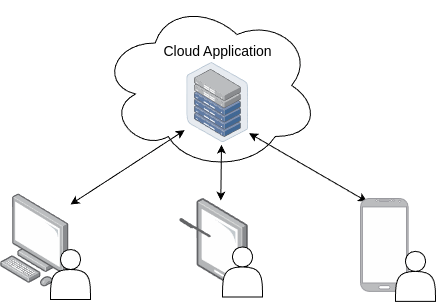
\includegraphics[scale=0.4]{images/basic-cloud-services.drawio.png}
    \caption{Cloud Application.}
    \label{fig:oauth:authcodeflow}
\end{figure}

\subsection{OpenID Connect}
\label{cha:relatedwork:openid}

% source: https://openid.net/specs/openid-connect-core-1_0.html

OpenID (OIDC for short) Connect is an identity layer built on top of the OAuth 2.0.
While OAuth 2.0 focuses on authorization (granting clients access to resources),
OIDC extends this to authentication.
Since OIDC deals with authentication, I will call the resource owner the user from now on.

% OIDC leverages the Authorization Code flow (described in Section \ref{cha:relatedwork:oauth:authcode}) of OAuth 2.0. However,
OIDC uses as its base either the Authorization Code flow
\ref{cha:relatedwork:oauth:authcode} or the Implicit flow
\ref{cha:relatedwork:oauth:implicit} and
it introduces a new type of token called an ID Token.
This ID Token is a JSON Web Token (JWT) that contains minimal information about the authenticated
user
Most importantly, the Id Token carries a Subject identifier, which is a unique identifier
for the user in the <- finish here 
The Id Token is sent alongside the Access token to the client, on which step this happens
depends on weather the Authorization Code flow or the Implicit flow is used.


% 3.2.1.  Implicit Flow Steps
% The Implicit Flow follows the following steps:
%
% Client prepares an Authentication Request containing the desired request parameters.
% Client sends the request to the Authorization Server.
% Authorization Server Authenticates the End-User.
% Authorization Server obtains End-User Consent/Authorization.
% Authorization Server sends the End-User back to the Client with an ID Token and, if requested, an Access Token.
% Client validates the ID token and retrieves the End-User's Subject Identifier.
% When using the implicit flow, the Id Token and, if requested, the Access Token
% are sent to the client after the user authenticated himself.
% After this the client could also use the Access Token to accsess 

In the OIDC flow, after the client obtains the Authorization Code,
it exchanges it for both an Access Token (as in OAuth 2.0) and an ID Token.
The client can then validate the ID Token to ensure it's genuine and extract the user information contained within.


% 3.1.1.  Authorization Code Flow Steps
% The Authorization Code Flow goes through the following steps.
%
% Client prepares an Authentication Request containing the desired request parameters.
% Client sends the request to the Authorization Server.
% Authorization Server Authenticates the End-User.
% Authorization Server obtains End-User Consent/Authorization.
% Authorization Server sends the End-User back to the Client with an Authorization Code.
% Client requests a response using the Authorization Code at the Token Endpoint.
% Client receives a response that contains an ID Token and Access Token in the response body.
% Client validates the ID token and retrieves the End-User's Subject Identifier.


% NOTE: maybe remove this
In essence, OIDC allows clients to obtain information about the authenticated user in a standardized way.

% TODO !!
\section{PROCEED's Assets}
\label{cha:relatedwork:proceed-assets}

Assets are Objects that users can create and manage through the MS's interface.
When referring to assets, we are only talking about the core features of the MS, not
objects that aid in the usage of the MS, like Roles .e.g., which only helps with managing
access to assets.
Currently the MS supports the following assets:

\begin{enumerate}
  \item Processes, Project and Templates: These objects store BPNN at their core.
  \item Task:
  \item Machine: Object that represents a server running Distributed Process Engine. The
    machine is used to manage properties of the server.
    % NOTE  maybe remove execution
  \item Execution: An execution represents a process that is being executed distributedly.
\end{enumerate}


\section{PROCEED's role system}
\label{cha:relatedwork:proceedroles}

The PROCEED MS uses a Role-Based Access Control %(RBAC) 
system to mange user authorization to determine what actions a user can perform.
Roles can be seen as bundles of permissions, which are granted to users.
A user can have multiple roles and all the permissions of the roles are additively
combined. That is, by adding a permission, a user can never do less than before.
Typically roles are assigned to users based on their job function.
%% Advantages 
%% - One role serves multiple people
%% - roles don't change ofte
%% - roles are easier to manage than individual permissions
RBAC can be advantageous since they can be assigned to multiple users and 
don't change often, making them easier to manage than individual permissions.

\subsection{MS's Role System Terminology}
\label{cha:relatedwork:proceedroles:terminology}

The following terms are important to understand the role system in the PROCEED MS:

\begin{itemize}
  \item Resource: A resource is any protected entity in the management system, that can be
    accessed by users.
  \item Action: An action is a specific operation that can be performed on a resource.
  \item Permission: A permission is a tuple of resource type and action, which specifies that a
    user can perform the action on the resource instances. Optionally a permission can have
    conditions that have to be met the by resource instances, for the user to be able to perform the action.
  \item Role: A role is a set of permissions. Roles can be assigned to users, which then
    inherit the role's permissions. Roles can have expiration dates, after which all
    permissions are revoked.
\end{itemize}

\subsection{MS's resources and actions}
\label{cha:relatedwork:proceedroles:ms-resources-actions}

The following are the resource types that are used in the PROCEED MS:
  \lstinline{Process}, 
  \lstinline{Project},
  \lstinline{Template},
  \lstinline{Task},
  \lstinline{Machine},
  \lstinline{Execution},
  \lstinline{Role},
  \lstinline{User},
  \lstinline{Setting},
  \lstinline{EnvConfig},
  \lstinline{RoleMapping},
  \lstinline{Share},
  \lstinline{Folder}.


These are the actions that can be performed on these resources:
  \lstinline{none},
  \lstinline{view},
  \lstinline{update},
  \lstinline{create},
  \lstinline{delete}.

\subsection{MS's roles in CASL}
\label{cha:relatedwork:proceedroles:casl}

The PROCEED MS uses \footnote{https://casl.js.org/v6/en/}{CASL} to implement Rules. CASL
is an isomorphic authorization JavaScript library.
To enforce authorization CASL has abilities, which are assigned to users.
Abilities expose functions to check weather a user can perform an action on a resource.
Abilities are defined by four parameters: user action, subject, fields, conditions.
User actions and subjects are analogous to actions and resources \ref{cha:relatedwork:proceedroles:terminology}.

CASL differentiates between subject type and subject instance. 
A subject instance is a specific instance of a subject type, e.g. a specific process
users are working on, is an instance of the resource type "Process". 

Fields are used to specify which fields of a resource instance an action can be performed
on, e.g. a user can update a process's name, but not its id, or creation date.

Conditions are used to specify additional conditions that have to be met by a resource
instance, for a user to be able to perform an action on it. E.g. a user can only update a
process if he created it.

\begin{lstlisting}[
  language=Javascript,
  style=codestyle,
  caption={CASL example},
]
import { defineAbility } from '@casl/ability';

class User {
  constructor(id) {
    this.id = id;
  }
}

class Process {
  constructor(user, name) {
    this.authorId = user.id;
    this.createdOn = new Date();
    this.name = name
  }
}

function abilityForUser(user){
  return defineAbility((can, cannot) => {
    can('delete', 'User', {id: user.id});

    can('update', 'Process', ['name'], {authorId: user.id});
  });
}

const user1 = new User(1);
const user1Ability = abilityForUser(user1);
const user1Process = new Process(user1, 'some process');

const user2 = new User(2);
const user2Ability = abilityForUser(user2);

user1Ability.can('update', 'Process'); // true
user1Ability.can('update', user1Process, 'name'); // true
user1Ability.can('update', user1Process, 'createdOn'); // false

user1Ability.can('delete', user1); // true
user1Ability.can('delete', user2); // false

user2Ability.can('update', 'Process'); // true
user2Ability.can('update', user1Process); //false
\end{lstlisting}

If there exist any possible resource instance, where the user has permission to perform an action,
then the user has permission to perform the action on the resource type.
E.g if a user has permission to view some process in the MS, then he has permission to view .
